%%%%%%%%%%%%%%%%%%%%%%%%%%%%%%%%%%%%%%%%%%%%%%%%%%%%%%%%%%%%%%%%%%%%%%%%%%%%%%%%
% event_selection.tex: Select of showering and tracking events:
%%%%%%%%%%%%%%%%%%%%%%%%%%%%%%%%%%%%%%%%%%%%%%%%%%%%%%%%%%%%%%%%%%%%%%%%%%%%%%%%
\chapter{Event Selection}
%\label{ch:event_selection}
The event selection is divided into sections, for events that have a boosted final state and events with a resolved final state.
The selection for each of these possible signal topologies are designed to be orthogonal and maximize total signal (resolved and boosted) over backgrounds as well as control-region creation. The selection criteria for the $ee$ and $\mu\mu$ channels are identical except for the triggers.


\section{Boosted Selection}

\subsection{Signal Region}

\begin{description}
\item[Boosted signal region:] \
  \begin{itemize}
  \item \textbf{$ee$ channel:} $ee$ triggers from Section~\ref{sec:triggers}.
  \item \textbf{$\mu\mu$ channel:} $\mu\mu$ triggers from Section~\ref{sec:triggers}.
  \item if 4 final state resolved objects found, then dR between the sub-leading muon and each AK4 jet $>0.4$: preserve orthogonality between boosted and resolved regions
  \item leading tight lepton with $\pt > \SI{60}{\GeV}$
  \item sub-leading loose lepton with $\pt >\SI{53}{\GeV}$
  \item at least one AK8 jet with  $\pt >\SI{200}{\GeV}$ \&\& $LSF > 0.7$ \&\& soft drop mass$ > \SI{40}{\GeV}$
  \item the sub-leading lepton must fall within the cone of the AK8 jet
  \item all leptons and jets with $|\eta| < 2.4$
  \item di-lepton mass $m_{ll} > \SI{200}{\GeV}$: to suppress DY+jets contribution
  \item $\Delta \phi > 2.0$ between selected jet and lead lepton
  \item $M_{l J} > \SI{600}{\GeV}$
  \end{itemize}
\end{description}

\subsection{Low $M_{lj}$ control region}

\begin{description}
\item[low $M_{lJ}$ boosted control region:]\ \\This is the control region used to check the \ttbar background prediction for our boosted analysis and derive a systematic uncertainty
  \begin{itemize}
  \item same as boosted signal region, but $M_{l j} < \SI{60}{\GeV}$
  \end{itemize}
\end{description}

\subsection{Flavor Sideband}

\begin{description}
\item[Boosted flavor sideband:]\ \\  This is the control region used to estimate the \ttbar contribution.
  \begin{itemize}
  \item \textbf{$ee$ channel} same as boosted $\mu\mu$ signal region but 1 leading muon and 1 secondary electron
  \item \textbf{$\mu\mu$ channel} same as boosted $ee$ signal region but 1 leading electron and 1 secondary muon
  \end{itemize}
\end{description}

\subsection{Z-mass Sideband}

\begin{description}
\item[low $M_{ll}$ boosted control region:]\ \\ This is the control region used to check the agreement between data and simulation on the DY contribution.
  \begin{itemize}
  \item same as boosted signal region, but
  \item di-lepton mass $m_{ll} < \SI{150}{\GeV}$
  \item no LSF requirement on AK8 jet
  \item no requirement that sub-leading lepton be contained within the AK8 jet
  \end{itemize}
\end{description}

\section{Resolved Selection}

\subsection{Signal Region}

\begin{description}
\item[Resolved signal region:] \
  \begin{itemize}
  \item \textbf{$ee$ channel:} $ee$ triggers from Section~\ref{sec:triggers}.
  \item \textbf{$\mu\mu$ channel:} $\mu\mu$ triggers from Section~\ref{sec:triggers}.
  \item leading tight lepton with $\pt > \SI{60}{\GeV}$
  \item sub-leading tight lepton with $\pt > \SI{53}{\GeV}$
  \item at least two AK4 jets with  $\pt > \SI{40}{\GeV}$
  \item all leptons and jets with $|\eta| < 2.4$
  \item di-lepton mass $m_{ll} > \SI{200} {\GeV}$: to suppress DY+jets contribution
  \item all objects $\Delta R > 0.4$ apart
  \item $M_{l l j j} > \SI{600}{\GeV}$
  \end{itemize}

\end{description}
\subsection{Low $M_{lljj}$ control region}

\begin{description}
\item[low $M_{lljj}$ resolved control region:]\ \\ This is the control region to check our ttbar background prediction for our resolved analysis and derive a systematic uncertainty
  \begin{itemize}
  \item same as resolved signal region, but $M_{l l j j} < \SI{600}{\GeV}$
  \end{itemize}
\end{description}

\subsection{Flavor Sideband}

\begin{description}
\item[Resolved flavor sideband:]\ \\  This is the control region used to estimate the \ttbar contribution.
  \begin{itemize}
  \item same as resolved $\mu\mu$ signal region but 1 leading electron and 1 sub-leading muon
  \end{itemize}
\end{description}

\subsection{Z-mass Sideband}

\begin{description}
\item[low $M_{ll}$ resolved control region:]\ \\ This is the control region to check the agreement between data and simulation on the DY contribution.
  \begin{itemize}
  \item same as resolved signal region, but
  \item di-lepton mass $m_{ll} < \SI{150}{\GeV}$
  \end{itemize}
\end{description}

\begin{figure}[htbp]
  \centering

  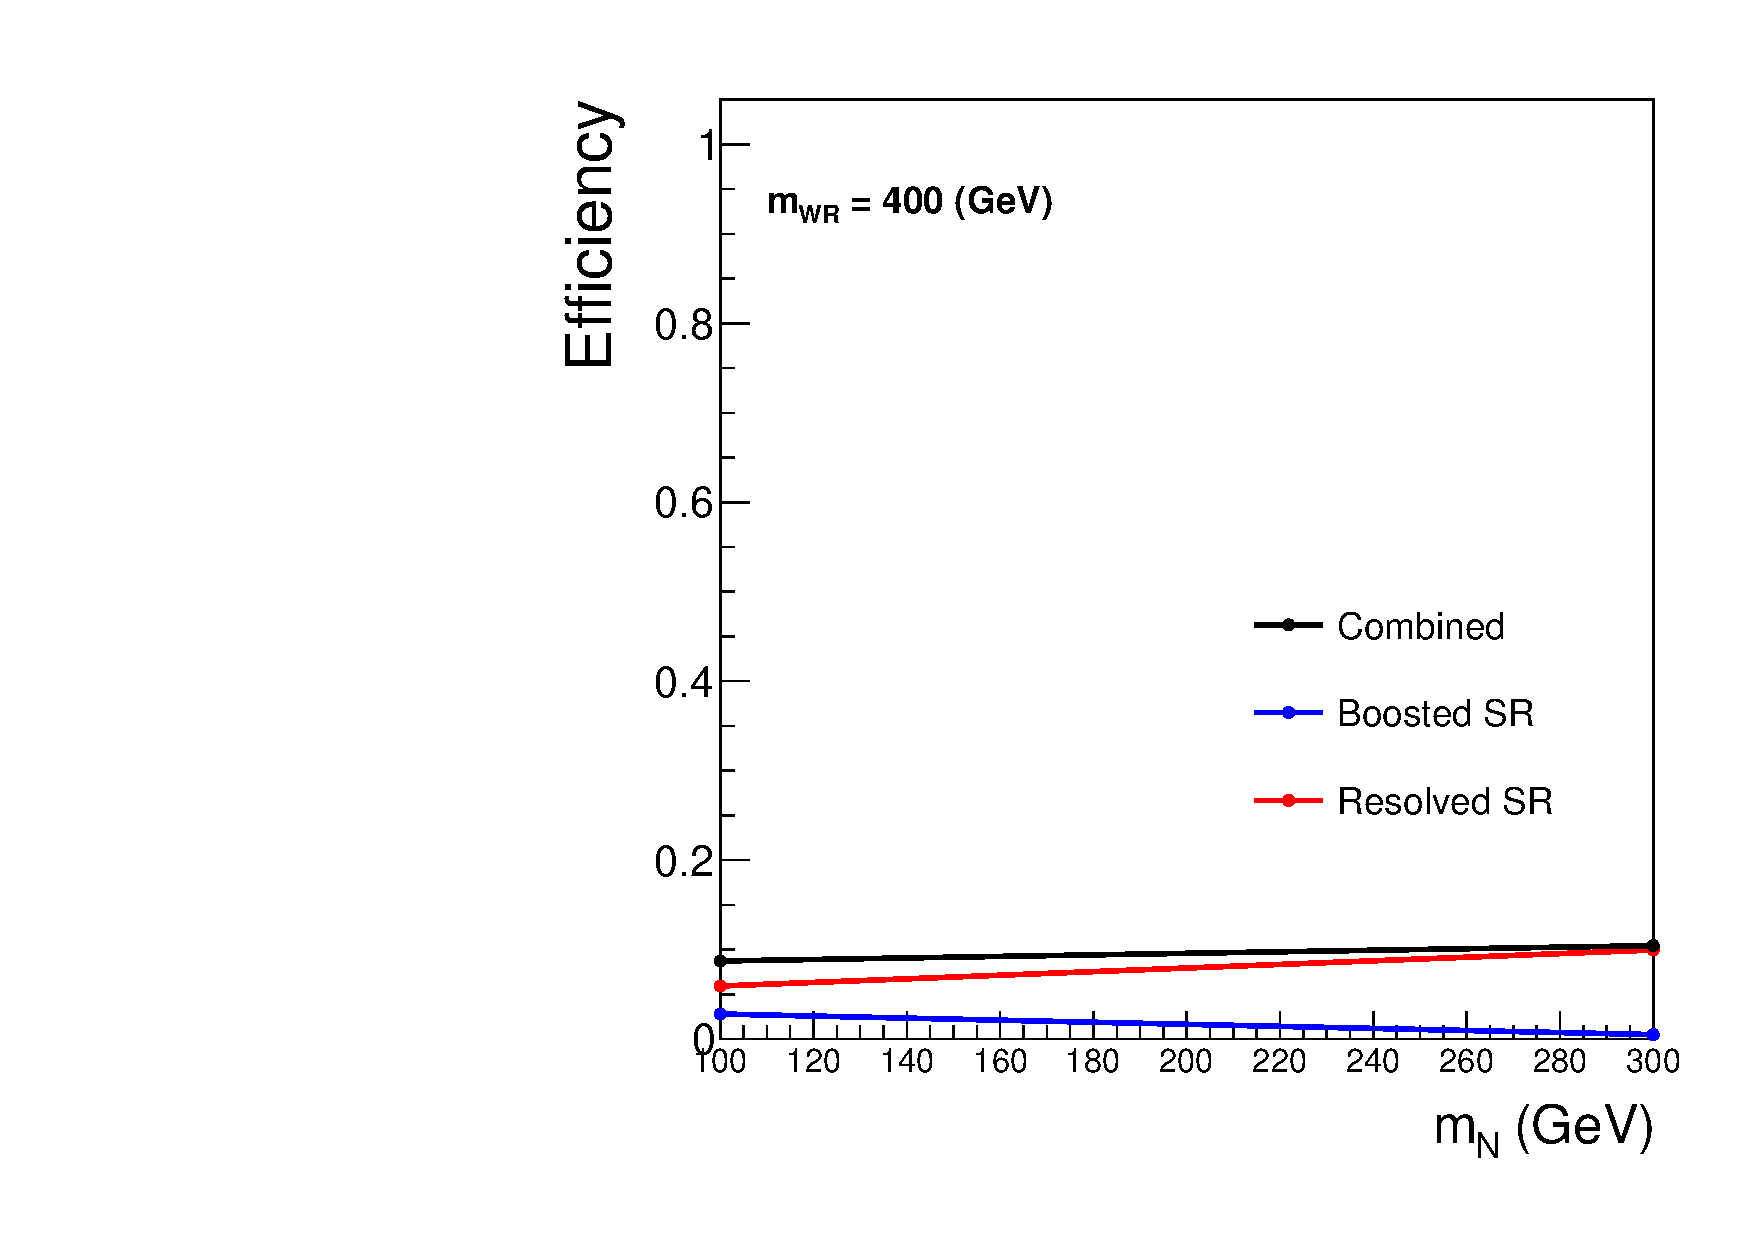
\includegraphics[width=0.45\textwidth]{figures/SigEff/WR400.pdf}
  \hspace{0.01\textwidth}
  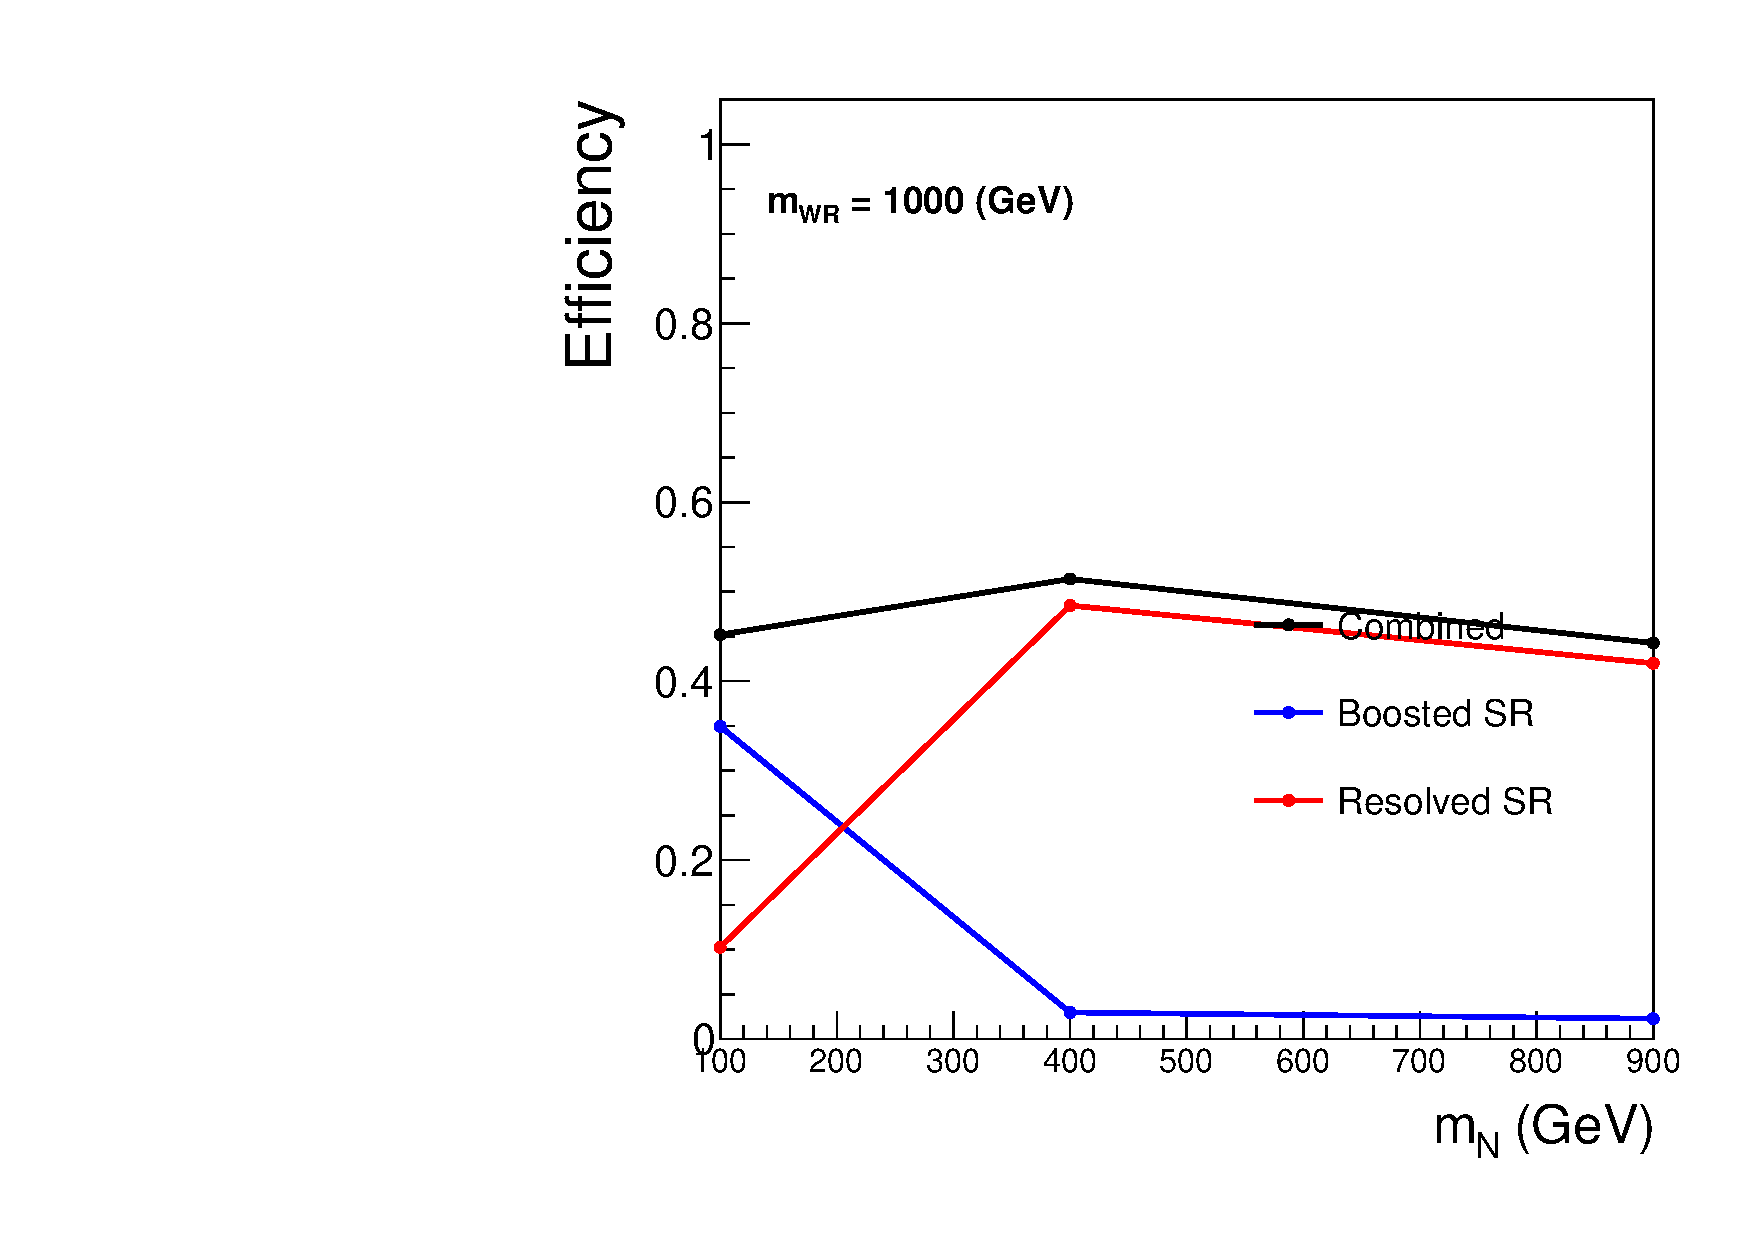
\includegraphics[width=0.45\textwidth]{figures/SigEff/WR1000.pdf}
  \vspace{0.01\textwidth}

  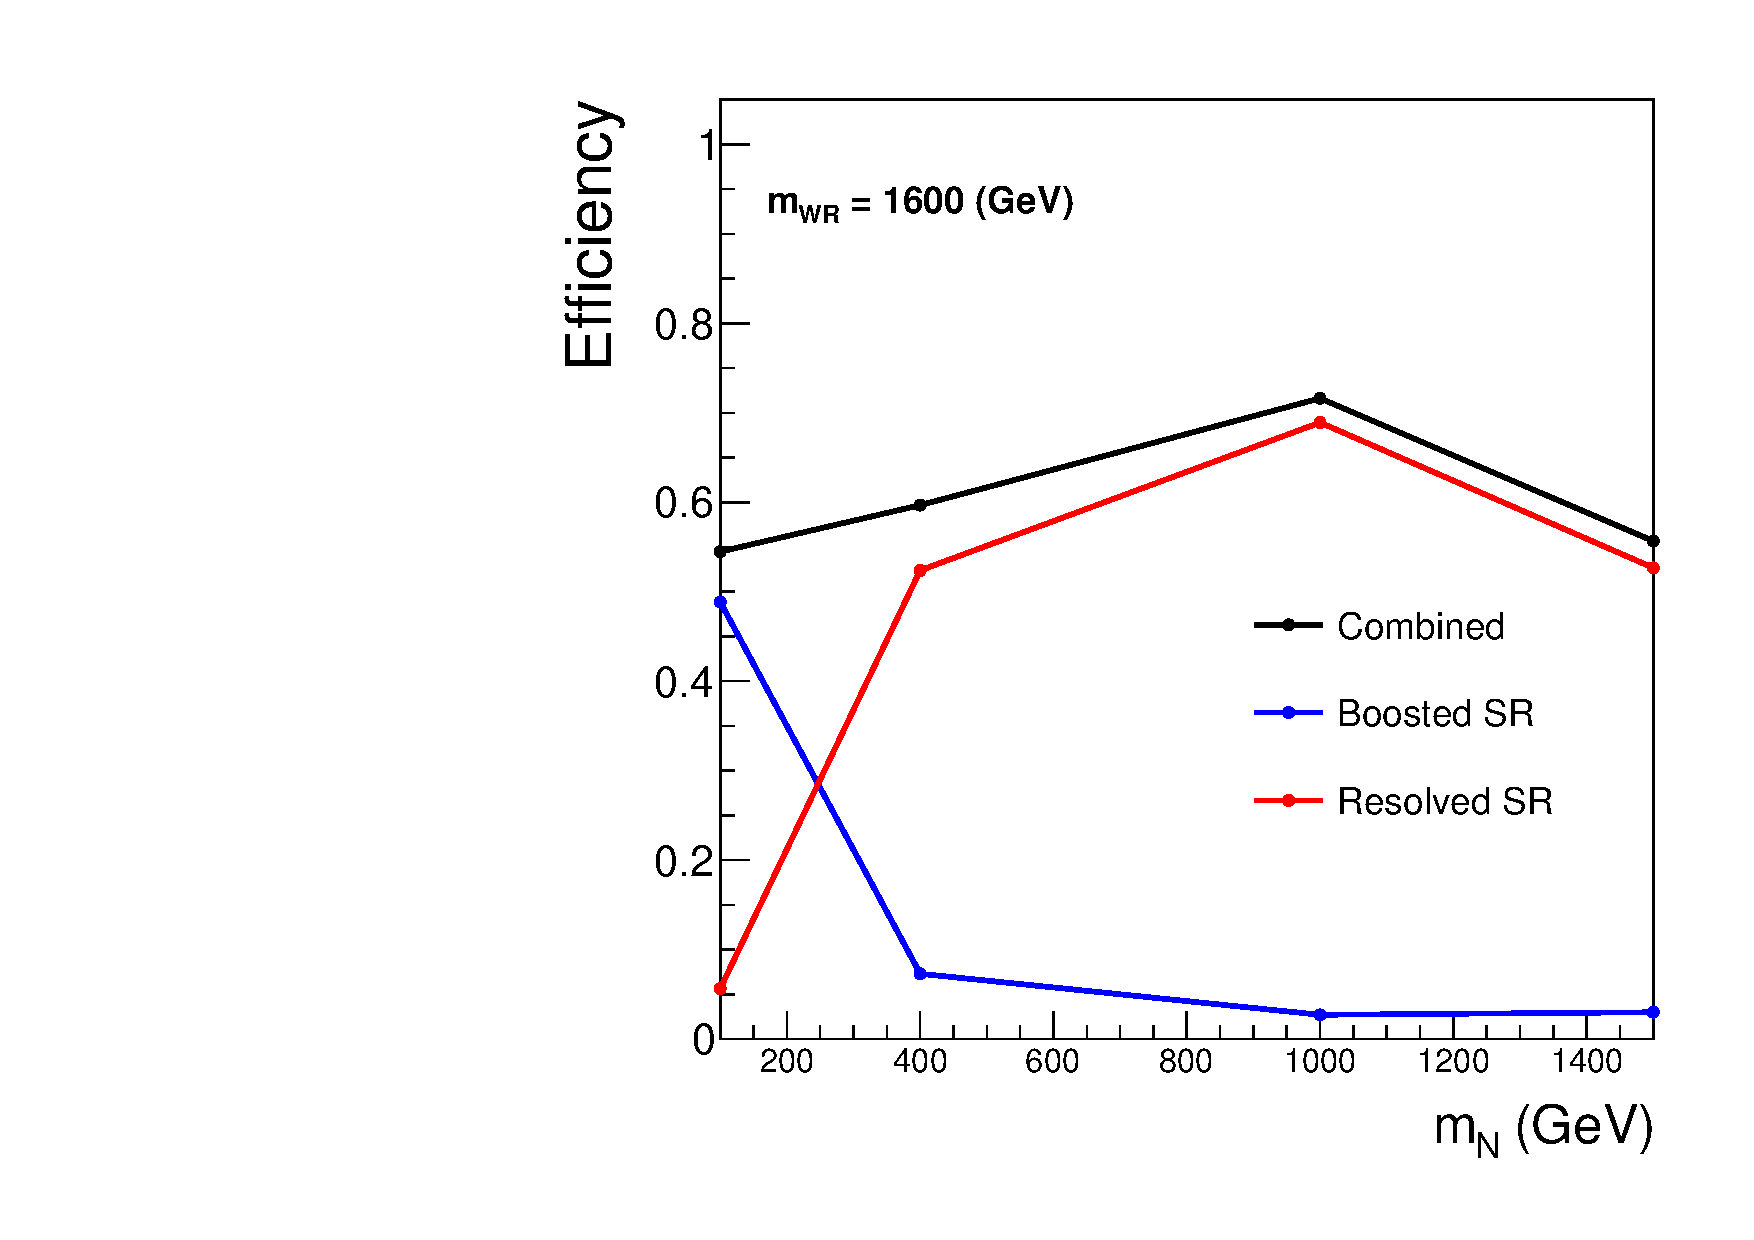
\includegraphics[width=0.45\textwidth]{figures/SigEff/WR1600.pdf}
  \hspace{0.01\textwidth}
  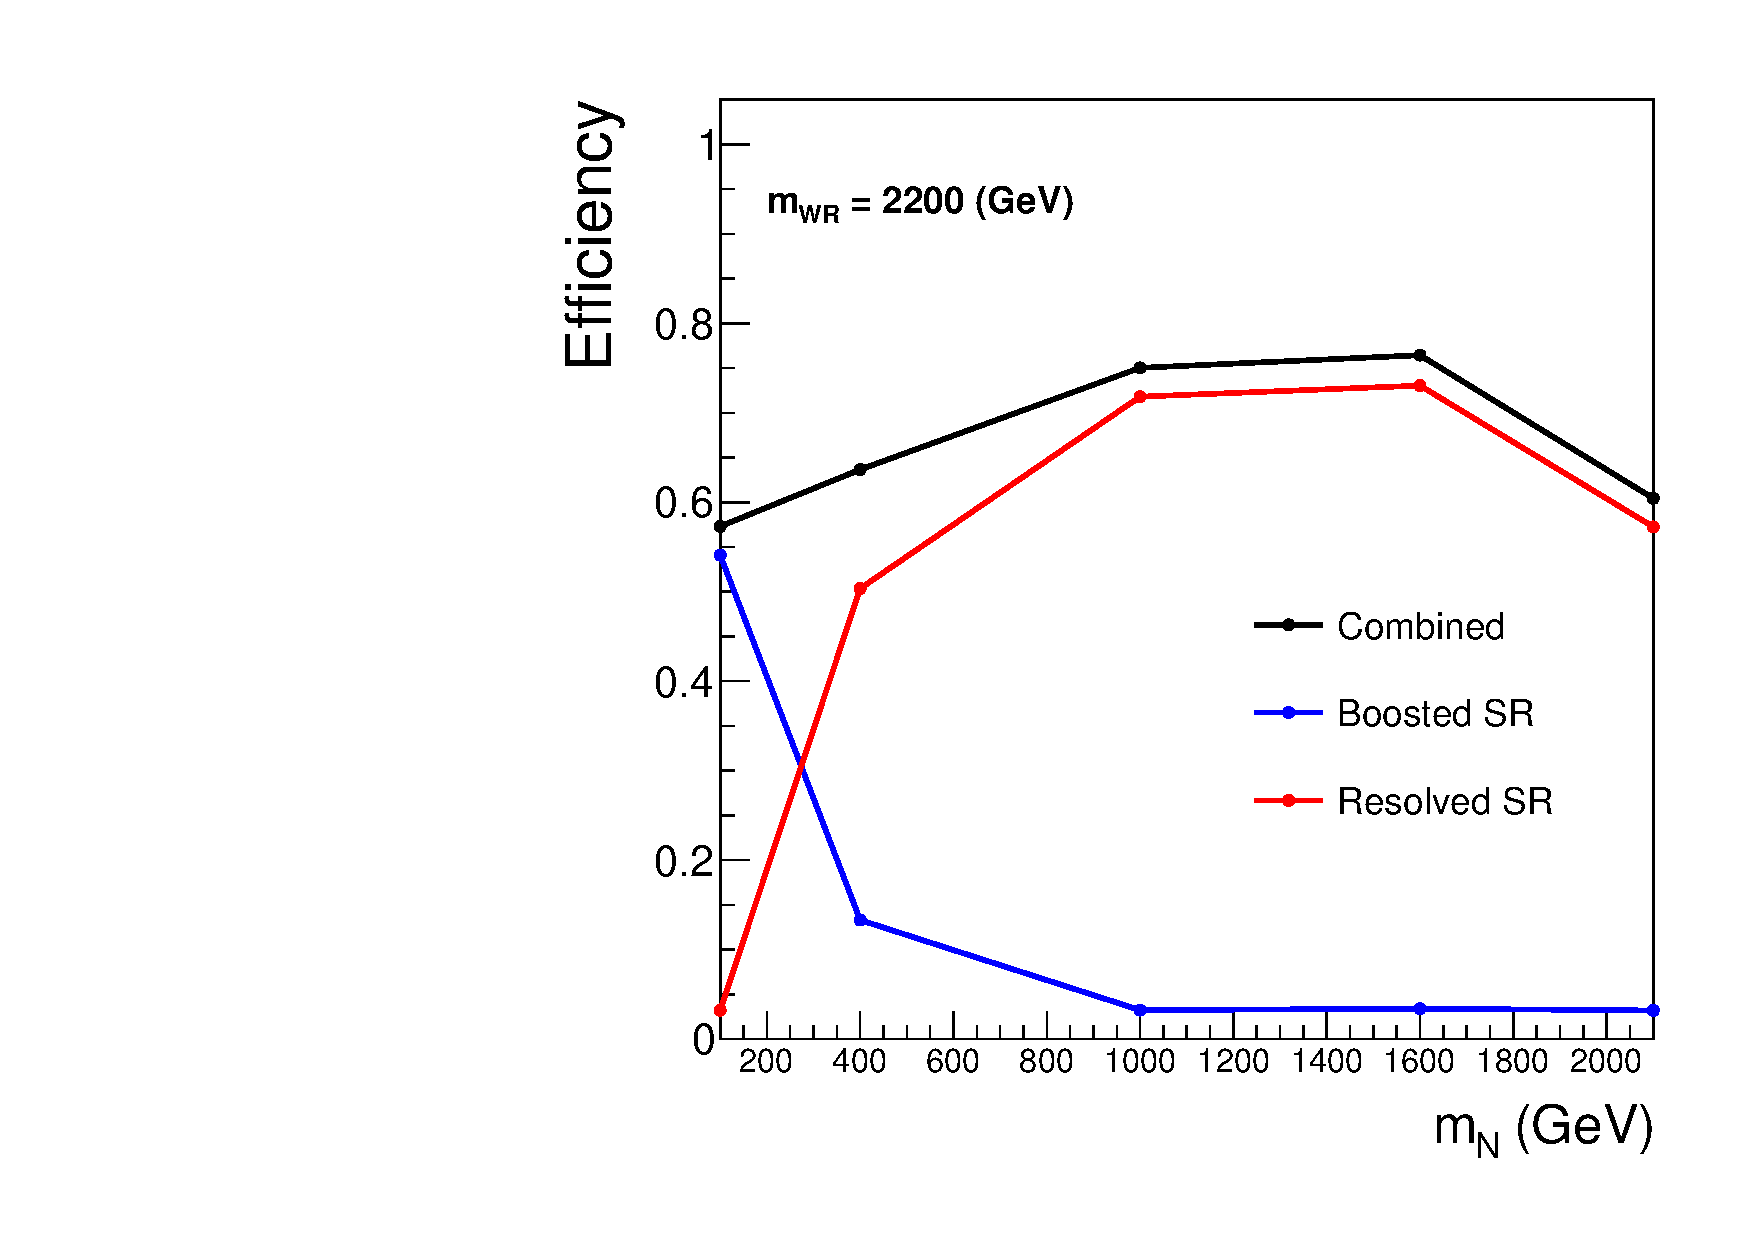
\includegraphics[width=0.45\textwidth]{figures/SigEff/WR2200.pdf}
  \vspace{0.01\textwidth}

  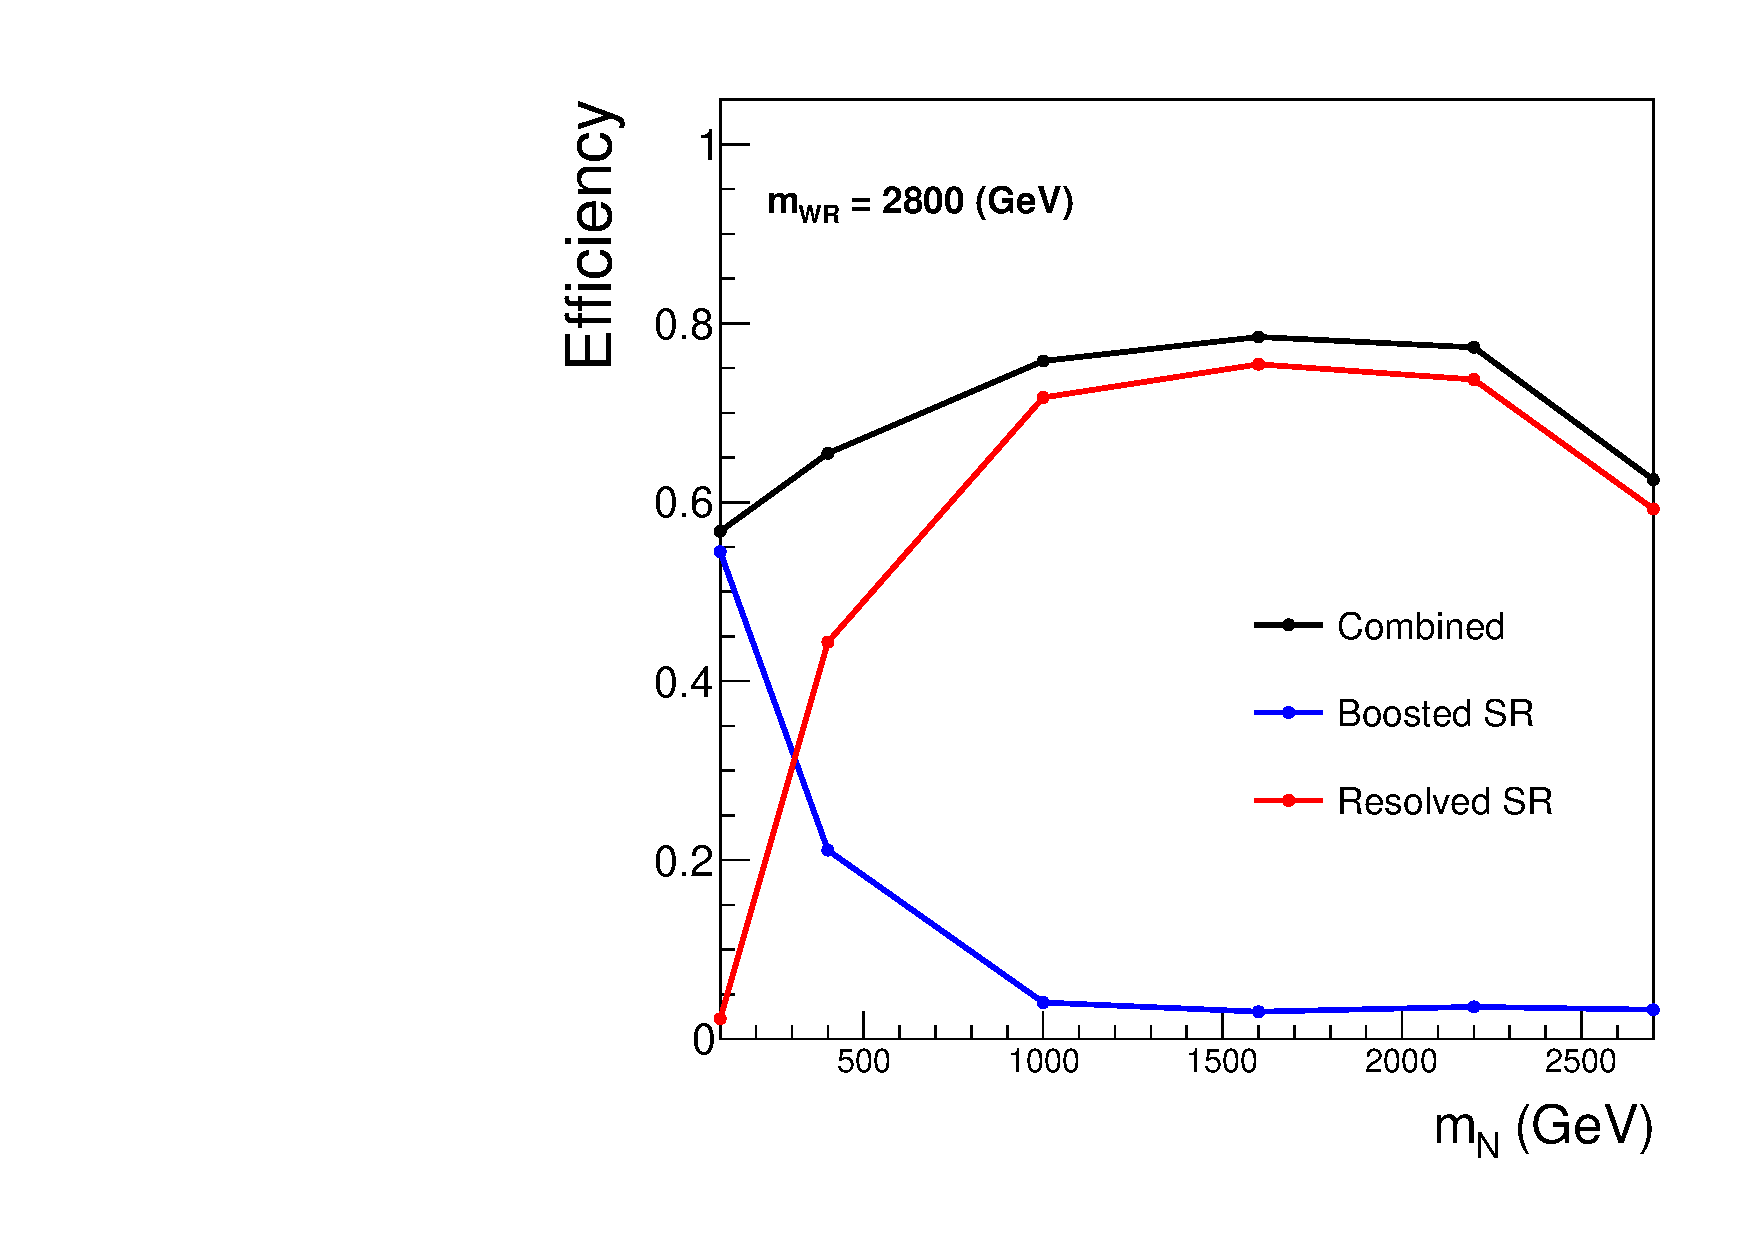
\includegraphics[width=0.45\textwidth]{figures/SigEff/WR2800.pdf}
  \hspace{0.01\textwidth}
  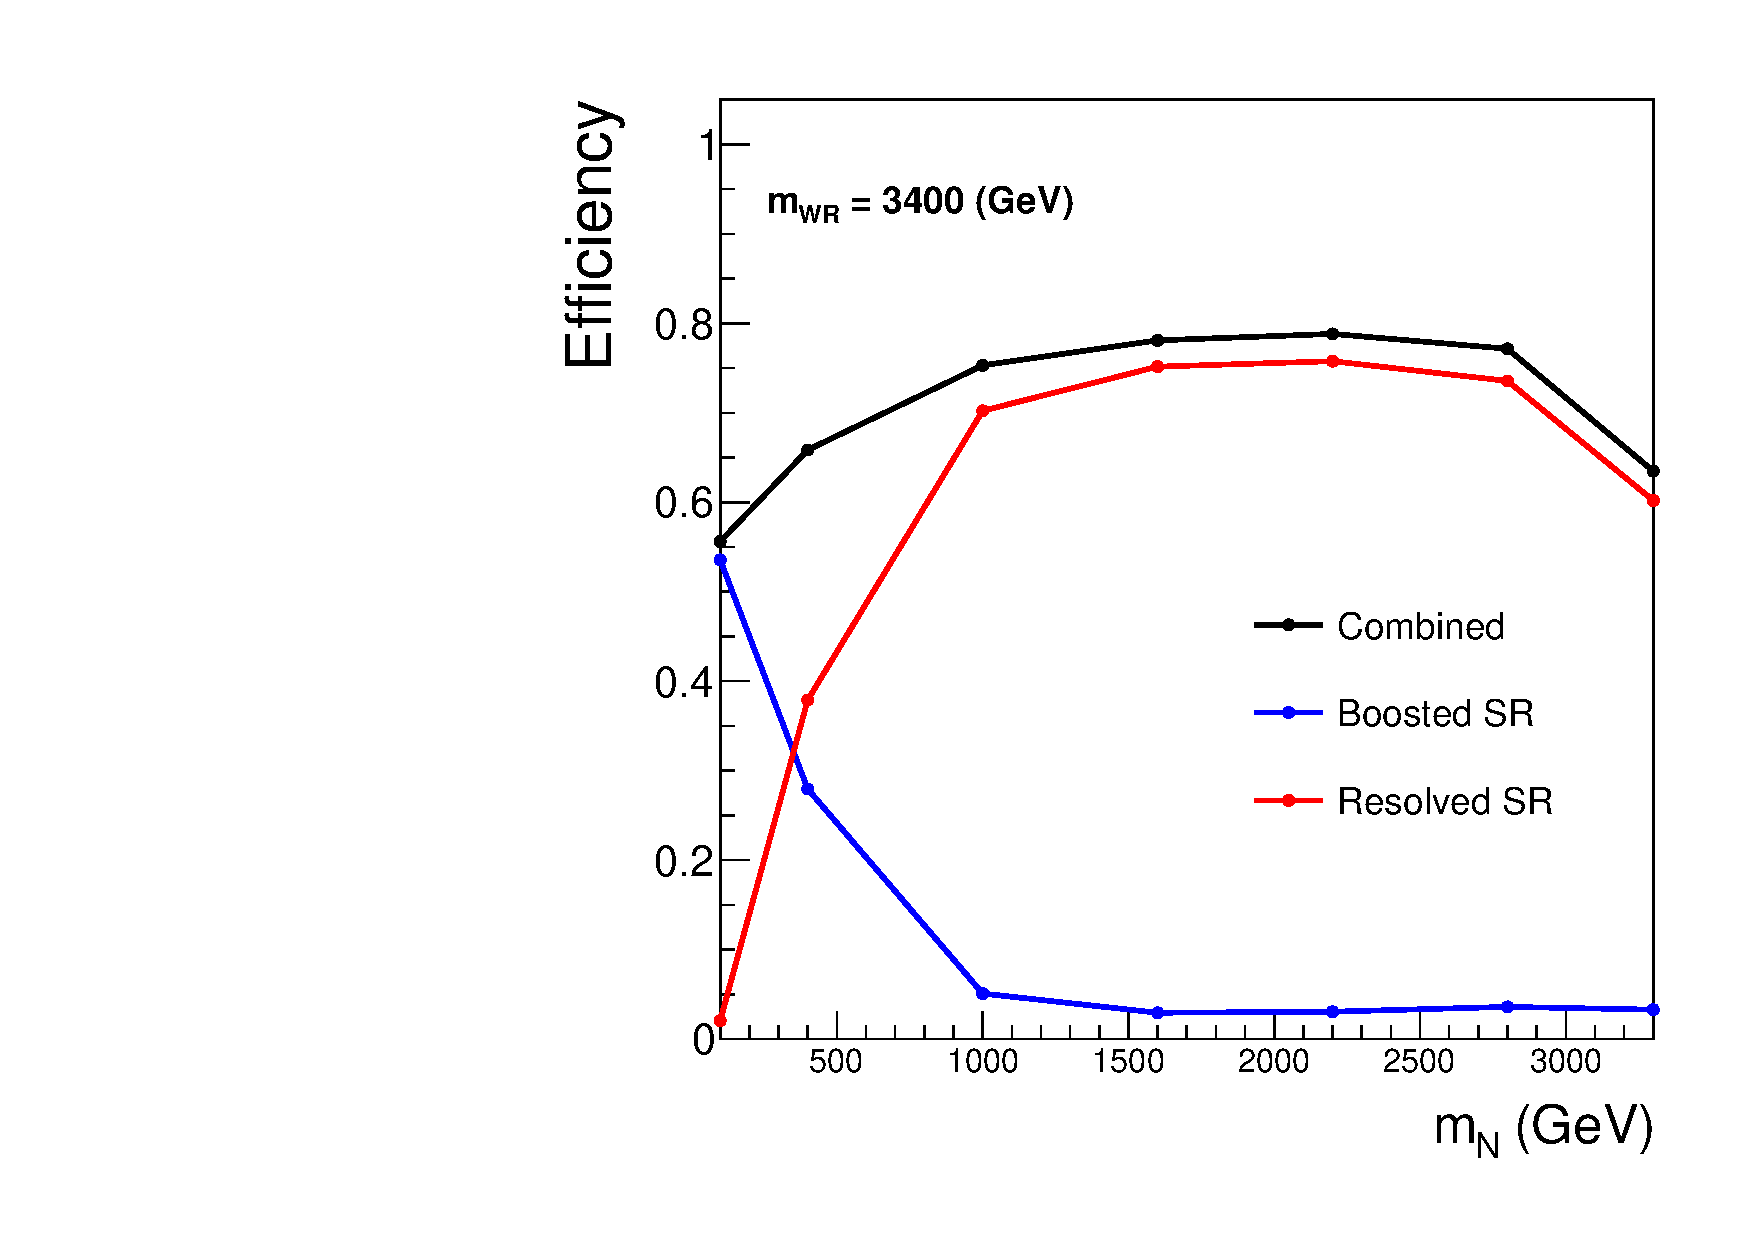
\includegraphics[width=0.45\textwidth]{figures/SigEff/WR3400.pdf}

  \caption[Signal Efficiencies for \MWR 400-3400]{
    The signal efficiencies in the signal regions (SR) for \WR masses of \ensuremath{\SI{400}{\GeV}-\SI{3400}{\GeV}}. In blue and red, the boosted and resolved signal region efficiency is shown respectively. The combined efficiency of each selection at a given mass point is shown as well. Efficiencies rise as the \WR mass rises into this analysis' selections. In all of them, it can be seen that the boosted signal regions reach peak efficiency at the lowest \NR mass points.
  }
  \label{fig:SigEff1}
\end{figure}

\begin{figure}[htbp]
  \centering

  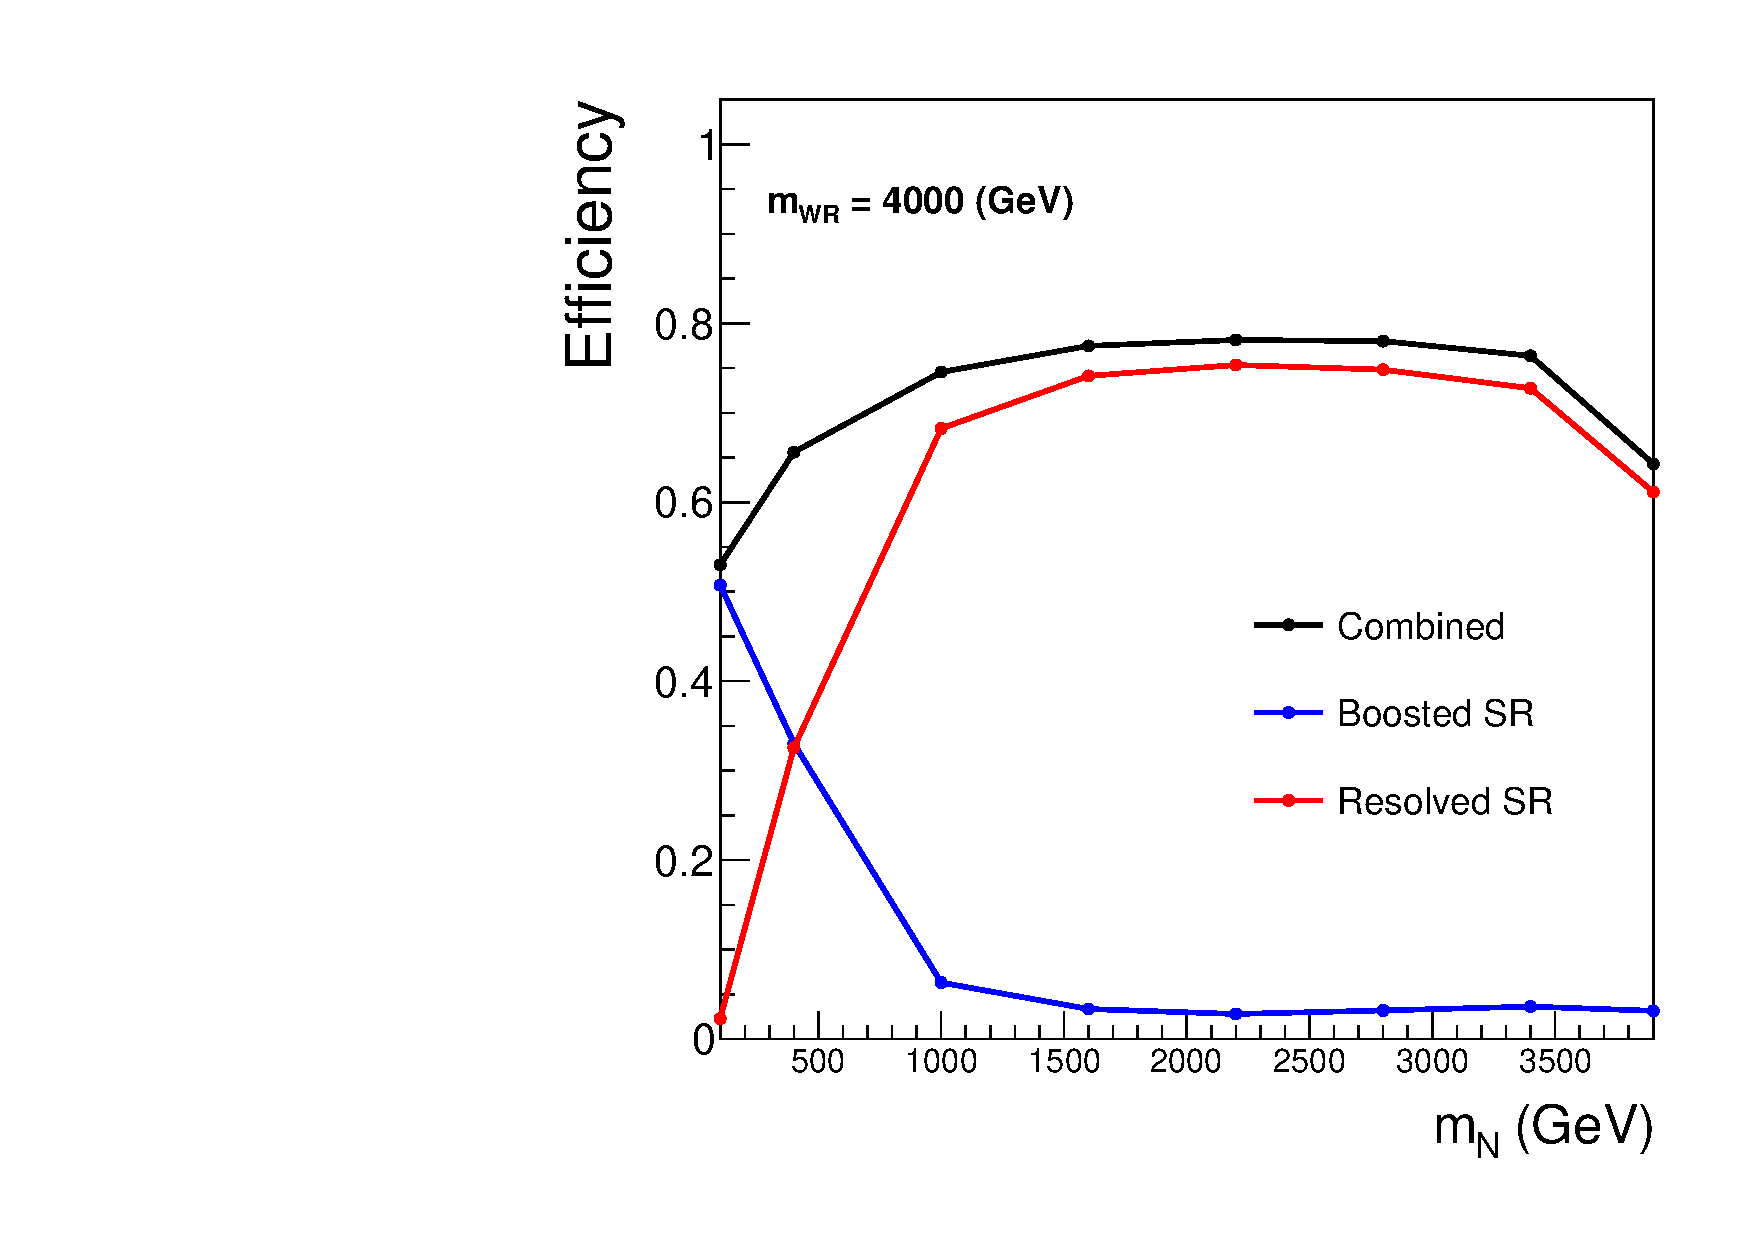
\includegraphics[width=0.45\textwidth]{figures/SigEff/WR4000.pdf}
  \hspace{0.01\textwidth}
  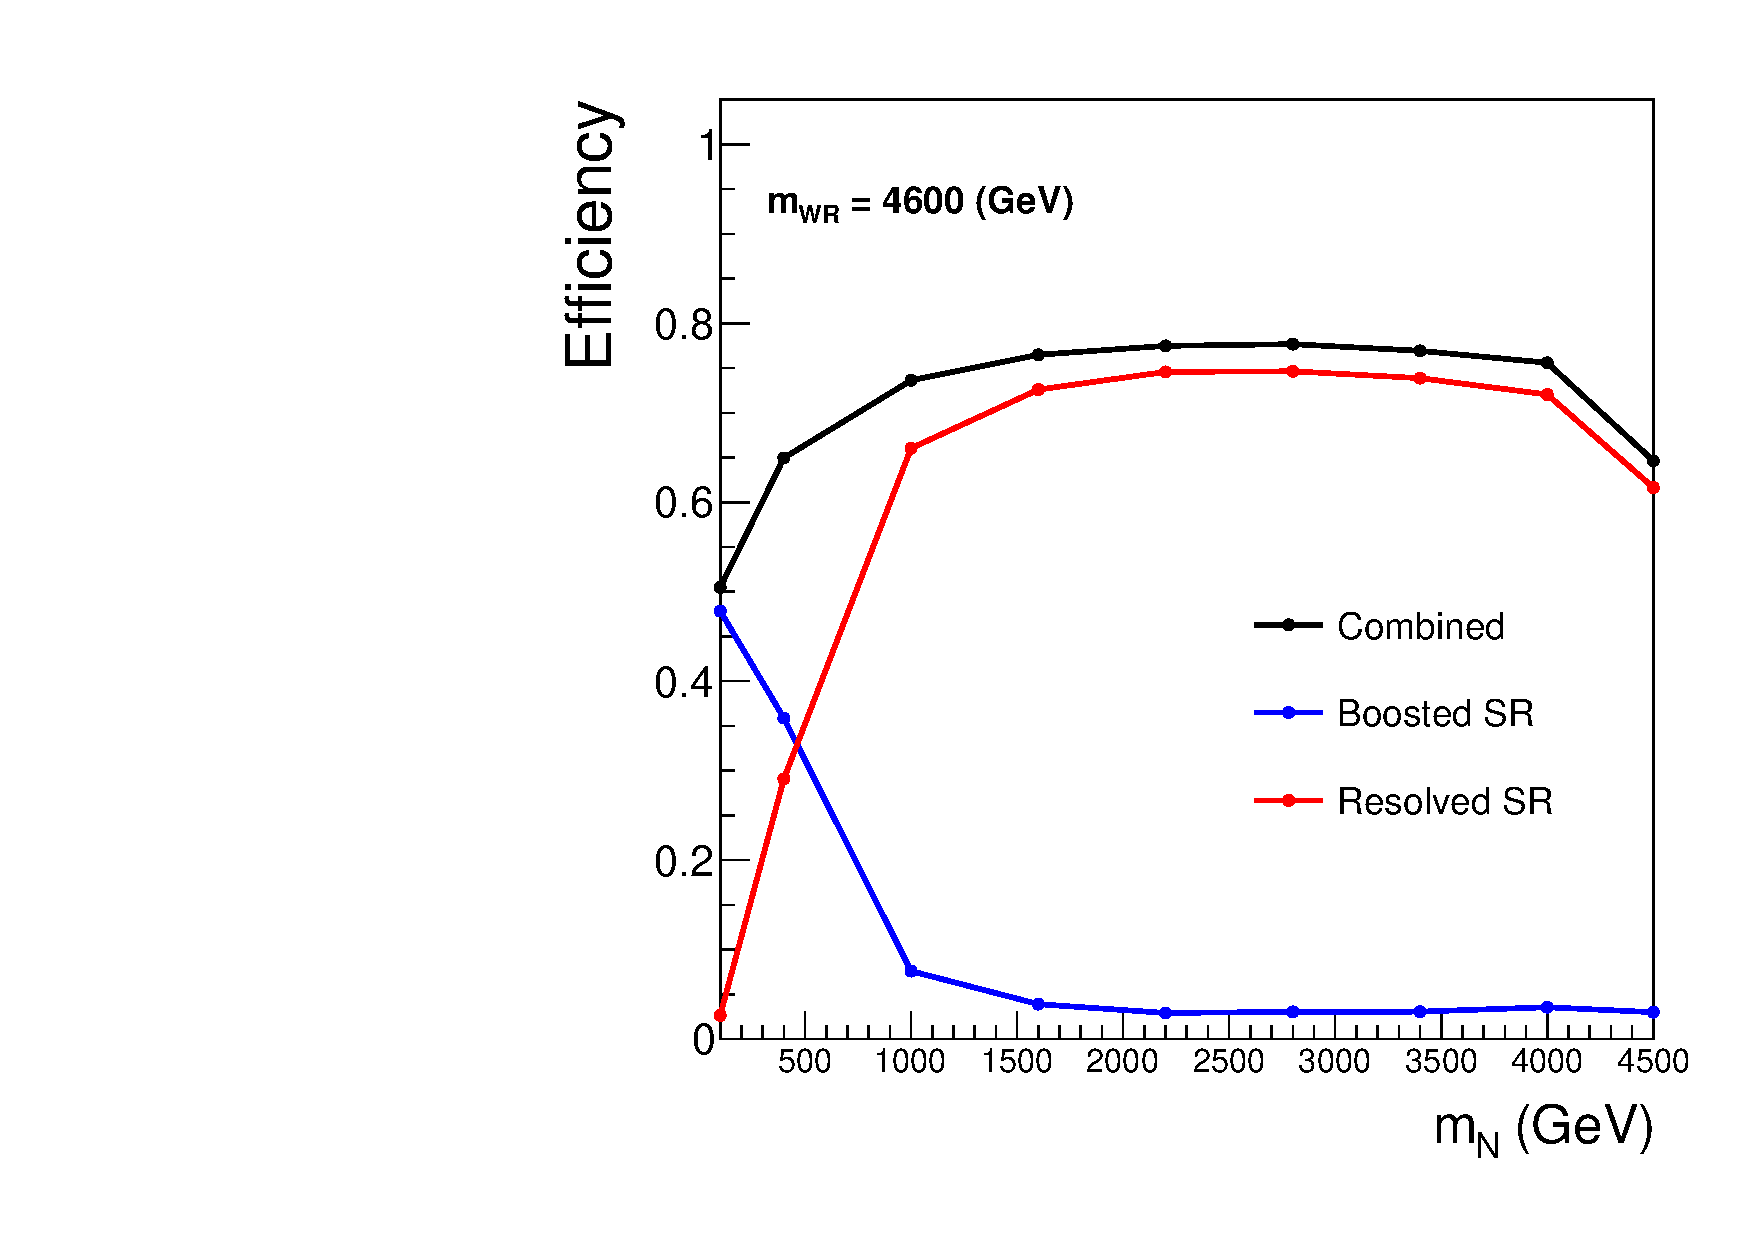
\includegraphics[width=0.45\textwidth]{figures/SigEff/WR4600.pdf}
  \vspace{0.01\textwidth}

  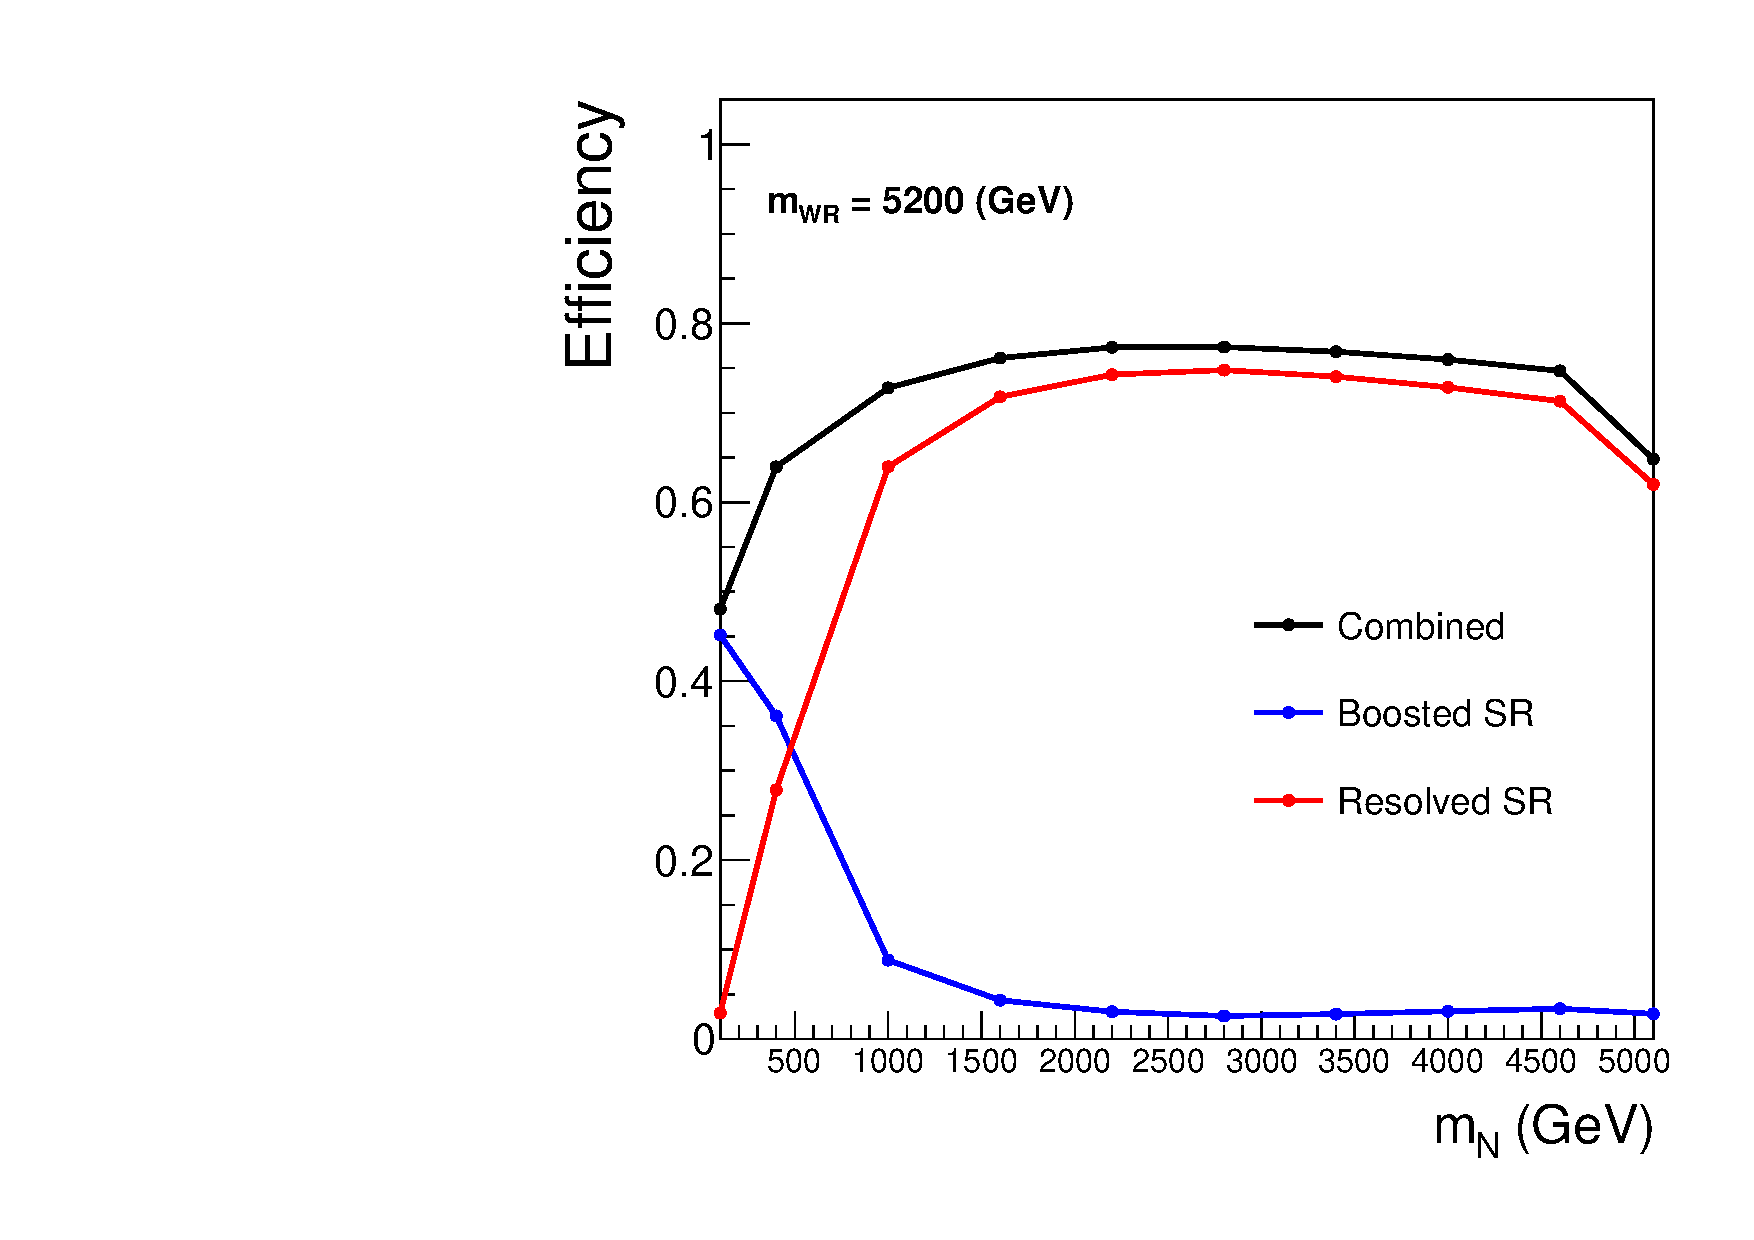
\includegraphics[width=0.45\textwidth]{figures/SigEff/WR5200.pdf}
  \hspace{0.01\textwidth}
  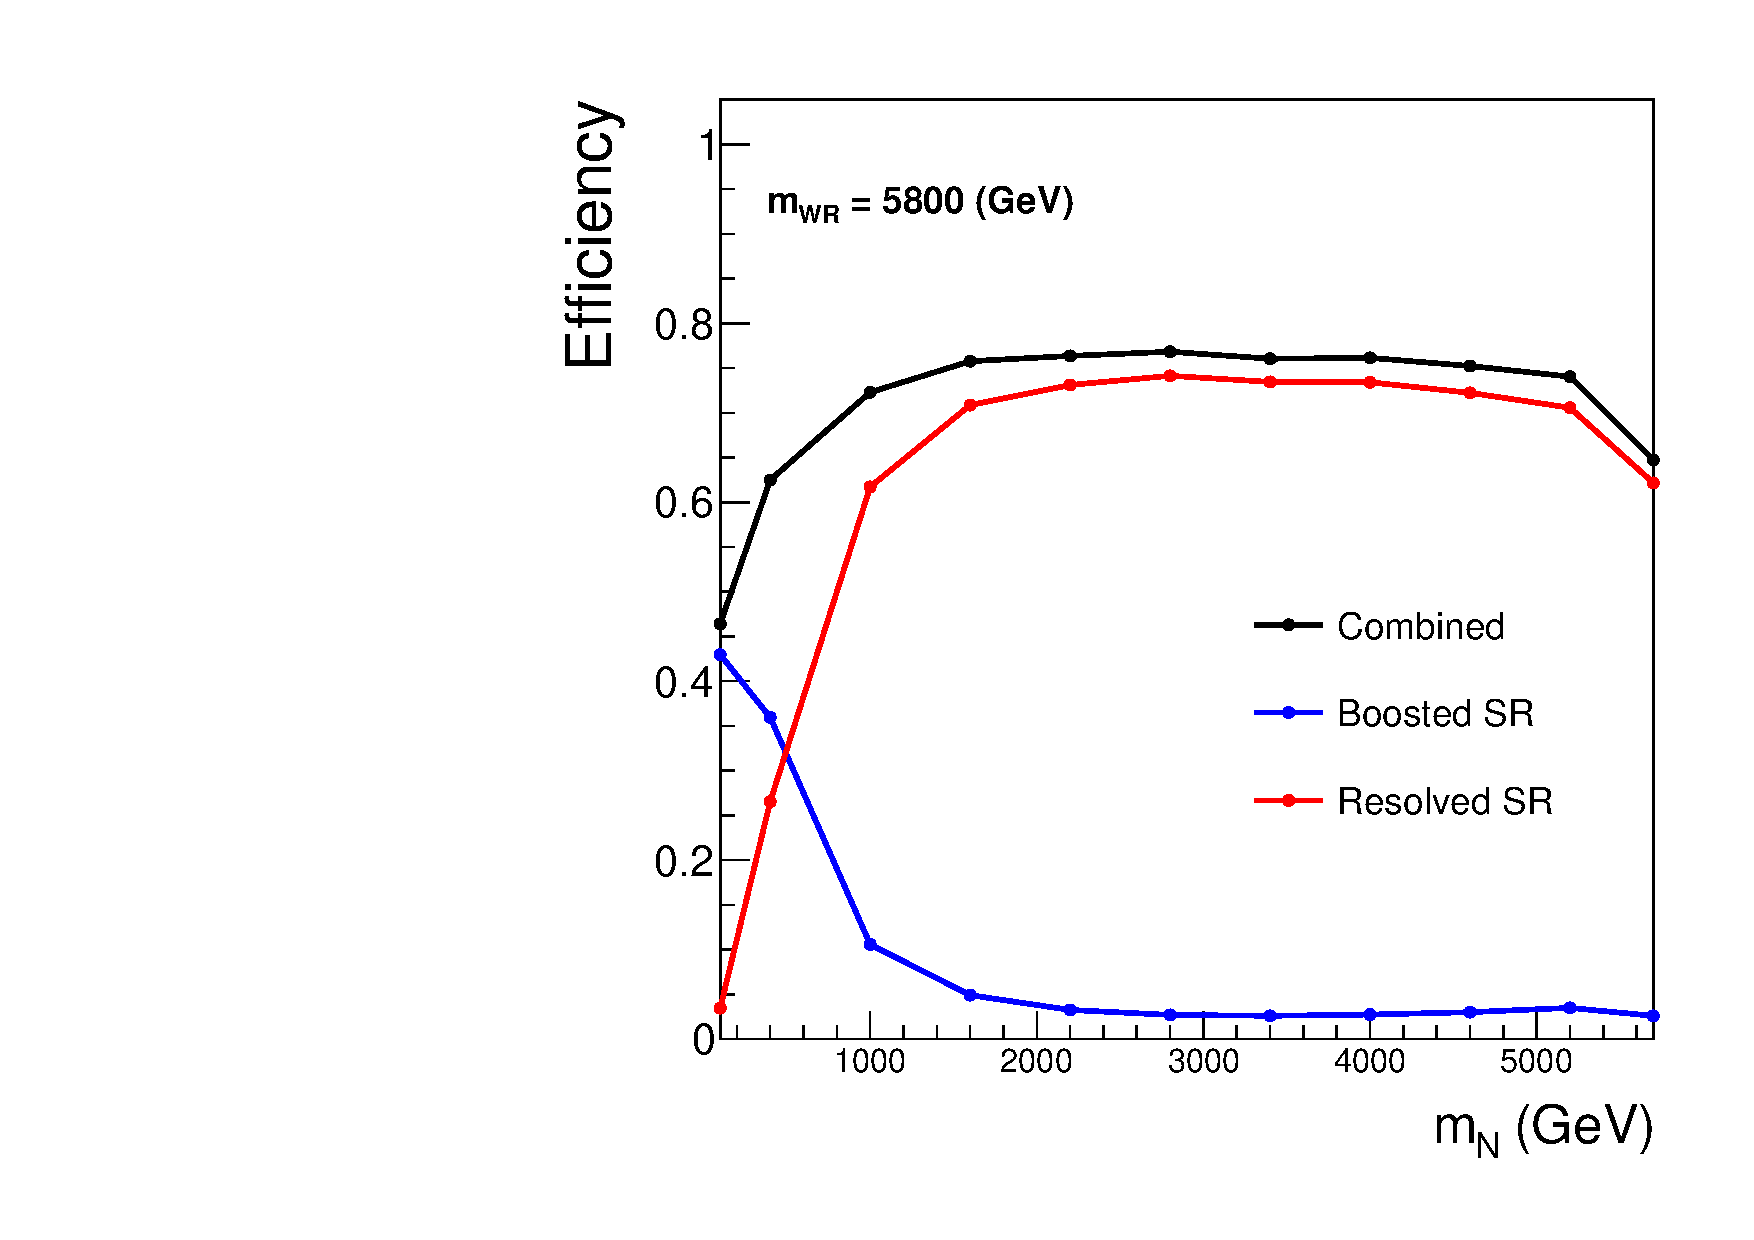
\includegraphics[width=0.45\textwidth]{figures/SigEff/WR5800.pdf}
  \vspace{0.01\textwidth}

  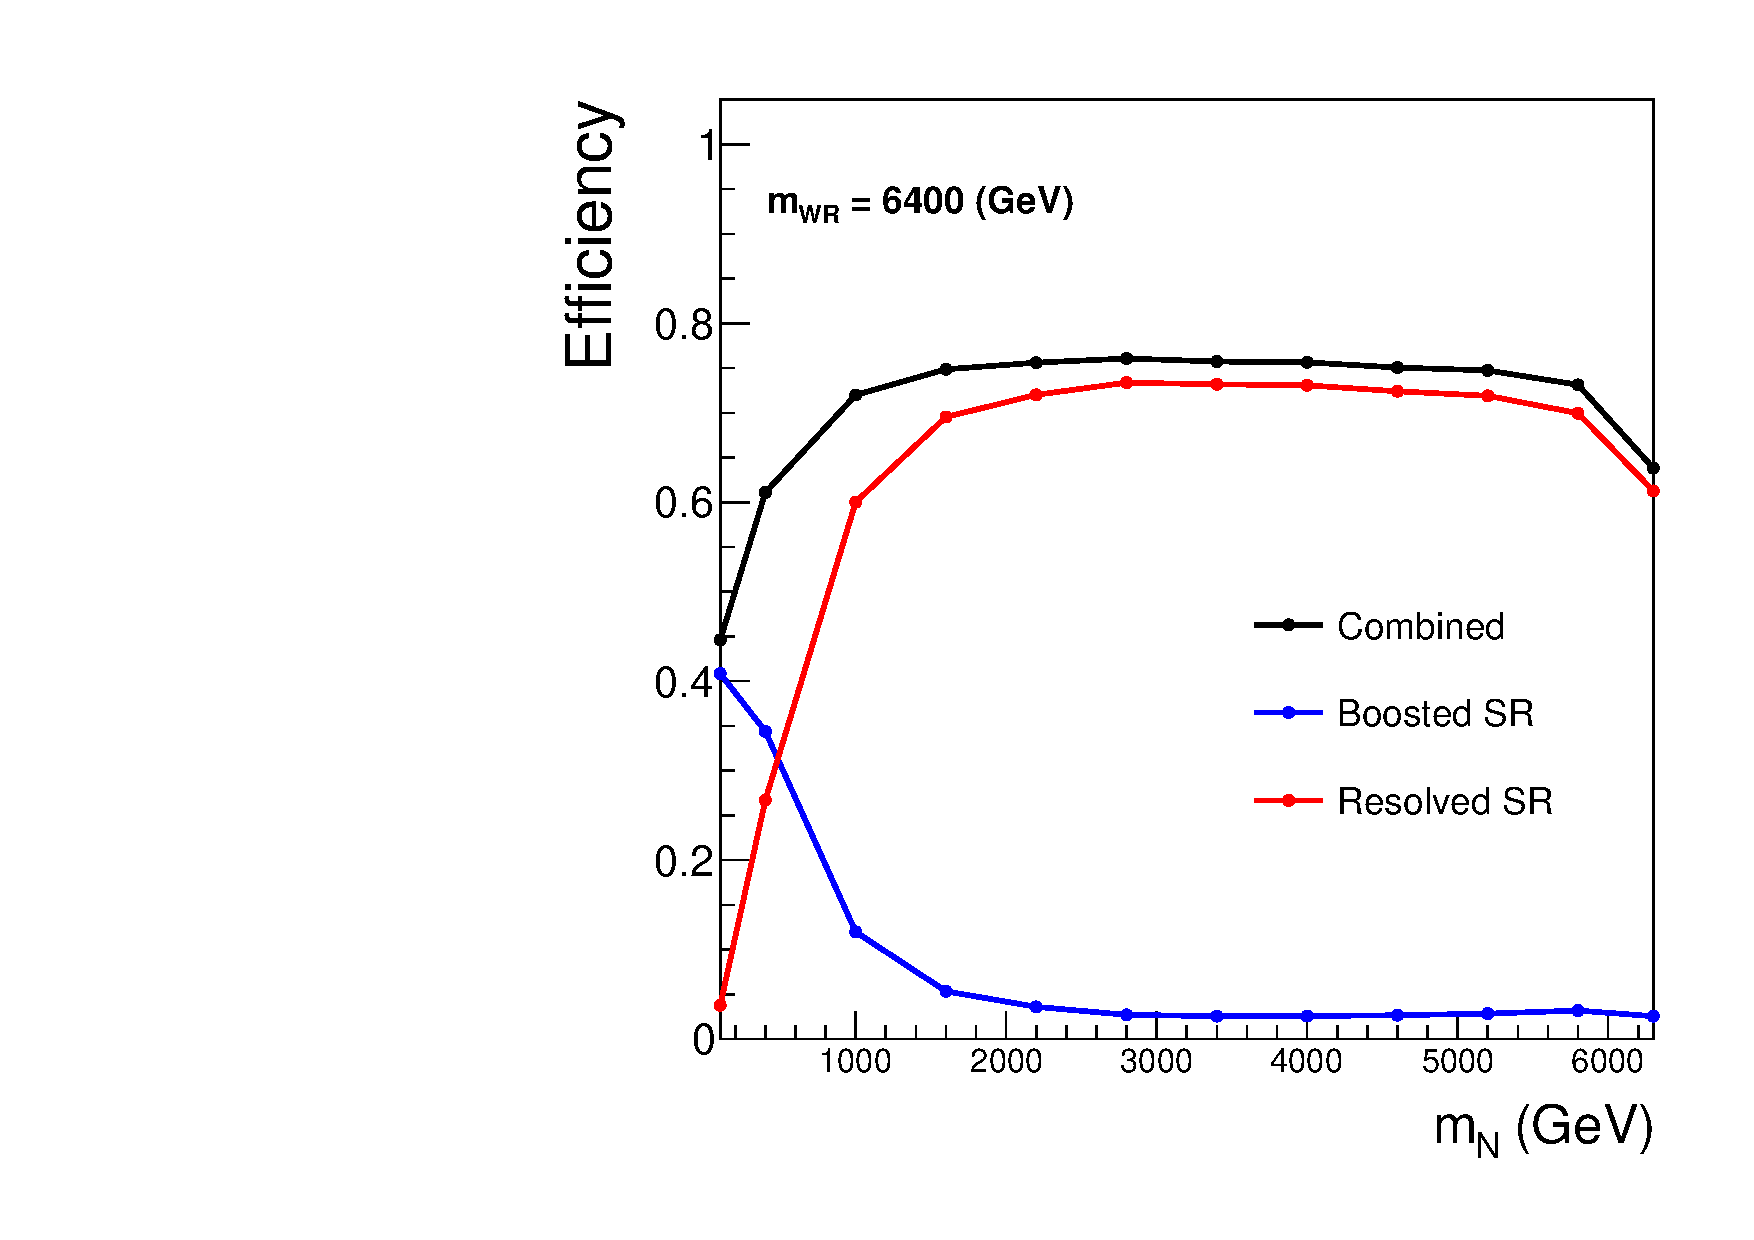
\includegraphics[width=0.45\textwidth]{figures/SigEff/WR6400.pdf}
  \hspace{0.01\textwidth}
  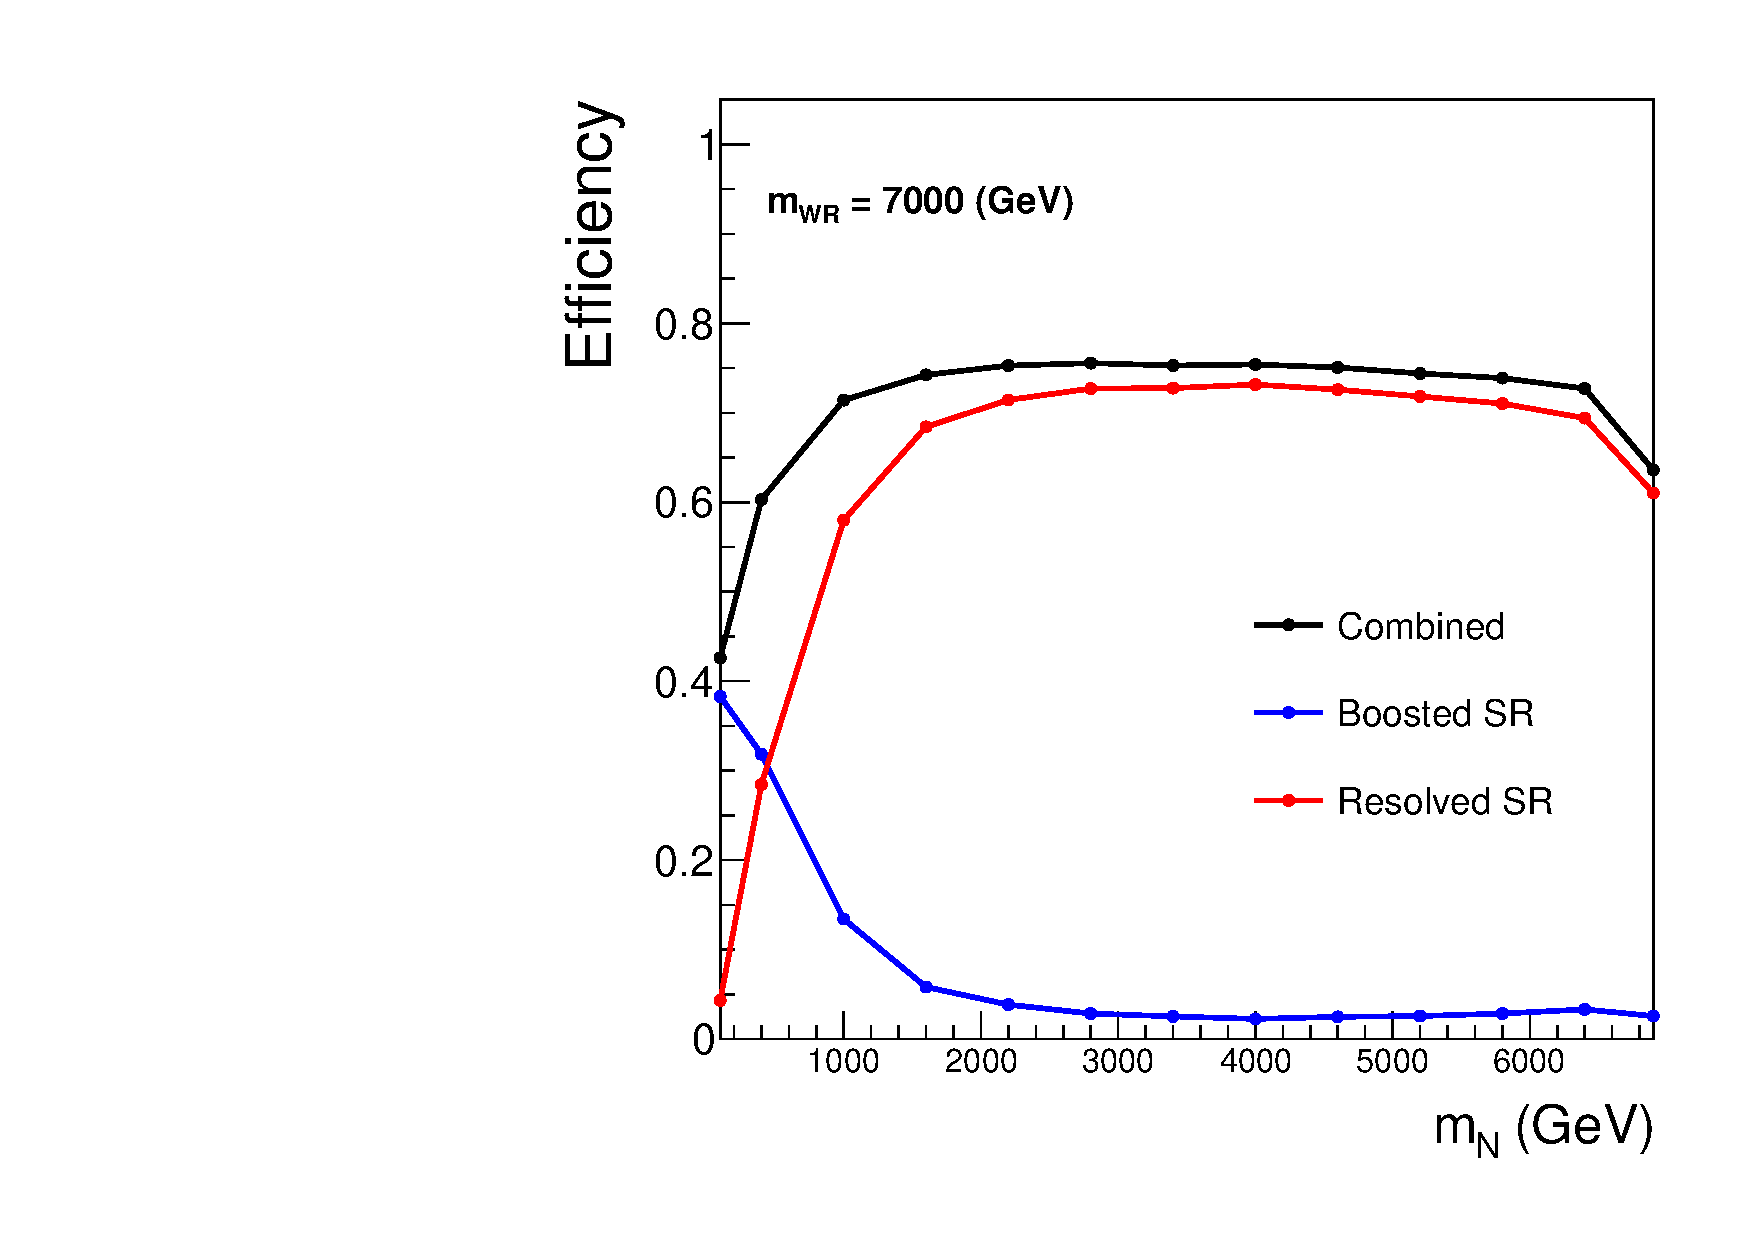
\includegraphics[width=0.45\textwidth]{figures/SigEff/WR7000.pdf}
  \caption[Signal Efficiencies for \MWR 4000-7000]{
    The signal efficiencies in the signal regions (SR) for \WR masses of \ensuremath{\SI{4000}{\GeV}-\SI{7000}{\GeV}}. In blue and red, the boosted and resolved signal region efficiency is shown respectively. The combined efficiency of each selection at a given mass point is shown as well. Efficiencies rise as the \WR mass rises into this analysis' selections. In all of them, it can be seen that the boosted signal regions reach peak efficiency at the lowest \NR mass points.
  }
  
  \label{fig:SigEff2}
\end{figure}

The reconstructed mass distributions of $W_{R}$ for the boosted and resolved signal regions is shown in \todo{use signal region plots} Fig~\ref{fig:BoostedSR} and~\ref{fig:ResolvedSR}, respectively.

\subsection{Signal efficiencies}
The signal efficiencies at the signal regions are shown in Fig.~\ref{fig:SigEff1}--\ref{fig:SigEff2},
as a function $m_{N}$, for each $m_{\WR}$.







%%%%%%%%%%%%%%%%%%%%%%%%%%%%%%%%%%%%%%%%%%%%%%%%%%%%%%%%%%%%%%%%%%%%%%%%%%%%%%%%

%%%%%%%%%%%%%%%%%%%%%%%%%%%%%%%%%%%%%%%%%%%%%%%%%%%%%%%%%%%%%%%%%%%%%%%%%%%%%%%%
